% !TeX program = pdflatex
% From the chromatic circle to the Tonnetz: the DFT as the eigenbasis of pitch-class symmetry.
% Author: Carles Marin (with Claude, Anthropic, as AI assistant).
% Style: first-tier mathematical-music-theory note -- restrained, question-driven, ONE BASIS as the
% connecting thread; plain booktabs tables with sparing semantic spot color; one-column serif.
% Note #3 in the music-math series (companion to sixthirty_note.tex and phase_taxonomy_note.tex).
% Build: pdflatex spectral_note.tex (twice, for refs).
% Source of record: research/music-math/paper/spectral_note.md (Curiosity, private repo).

\documentclass[11pt]{article}
\usepackage[T1]{fontenc}
\usepackage{lmodern}
\usepackage{amsmath,amssymb,amsthm,booktabs,graphicx}
\usepackage[hidelinks]{hyperref}
\usepackage{xurl}
\usepackage[table]{xcolor}
\usepackage[margin=1in]{geometry}
\usepackage{microtype}
\usepackage{float}
\usepackage[section]{placeins}
\usepackage{float}
\definecolor{ctA}{HTML}{1B6F8C} % the "abelian / augmented" accent
\definecolor{ctB}{HTML}{B5530F} % the "diminished / tritone" accent
\setlength{\emergencystretch}{2em}
\newtheorem{theorem}{Theorem}
\newtheorem{proposition}{Proposition}
\newtheorem{remark}{Remark}
\newcommand{\lean}[1]{\texttt{#1}}
\newcommand{\qlink}[1]{\par\medskip\begin{quote}\itshape\small\color{ctB!88!black}#1\end{quote}\medskip}
\newcommand{\Ztwelve}{\mathbb{Z}_{12}}
\newcommand{\Zn}[1]{\mathbb{Z}_{#1}}
\newcommand{\dft}{\mathcal{F}}
\newcommand{\Ahat}{\hat{A}}
\newcommand{\question}[1]{\smallskip\noindent\textit{#1}\smallskip}

\title{\bf The Tonnetz spectrum is the generating triad's\\ Fourier balance profile\\[5pt]
\large\rm a machine-checked DFT account of pitch-class symmetry,\\ from the chromatic circle to the neo-Riemannian Tonnetz}
\author{Carles Mar\'in\thanks{Prepared with the assistance of an AI system (Claude, Anthropic).
The mathematics is classical; every claim, scope statement, and limitation is the author's
responsibility, and the Lean~4 kernel---not the assistant---is what certifies the formalized parts.
The boundary of the contribution is stated plainly in Section~\ref{sec:novelty}.}\\[3pt]
  \normalsize Independent researcher\\
  \normalsize \texttt{karlesmarin@gmail.com}}
\date{June 2026\\[3pt]\normalsize DOI: \href{https://doi.org/10.5281/zenodo.20862822}{10.5281/zenodo.20862822}
\quad\textbullet\quad \href{https://github.com/karlesmarin/music-math}{github.com/karlesmarin/music-math}}

\begin{document}
\maketitle

\begin{abstract}\noindent
The neo-Riemannian \textbf{Tonnetz} --- the graph on the $24$ major and minor triads joined by the
parsimonious $P,L,R$ moves --- has an adjacency spectrum, and our main result identifies it exactly:
\textbf{the eigenvalues of the Tonnetz are $\pm$ the Fourier balances of the single triad that generates
it}, the signed set of distinct eigenvalues $\pm\{3,\sqrt5,\sqrt3,1,2\cos\frac{\pi}{12},2\cos\frac{5\pi}{12}\}
=\{\pm|\hat{\mathbf 1}_T(k)|\}_{k=0}^{6}$ ($|a_2|=|a_6|=1$ coincide). The augmented balance $\sqrt5=|a_3|$, the diminished
$\sqrt3=|a_4|$, the whole-tone $1=|a_6|$ --- the chord's own periodicity weights --- are literally the
graph's vibration frequencies (Theorem~\ref{thm:main}). We prove it by building the one tool that makes it
inevitable: the discrete Fourier transform is the shared eigenbasis of pitch-class symmetry.
(i)~every translation-invariant operator on $\Zn{N}$ (the chromatic cycle $C_{12}$, every abelian Cayley
graph) is \textbf{diagonalized} by the DFT characters, eigenvalue the Fourier coefficient of its connection
set (Babai). (ii)~adjoining inversion makes the $T/I$ group $D_{2N}$ \textbf{block-diagonal}, pairing
$a_k\leftrightarrow a_{-k}$ into conjugate-pair irreducibles. (iii)~the Tonnetz is the Cayley graph of the
non-abelian $PLR\cong D_{12}$ group, and reading it through (i)--(ii) yields the balance-profile identity,
\emph{complete with multiplicities}. Every step is machine-checked in Lean~4, sorry-free and axiom-clean ---
including the unconditional \textbf{completeness} of the spectrum (an explicit basis of eigenvectors; no
Sage, no irrep classification). The spectral formula itself is standard --- the dihedral-Cayley computation
of Gao--Luo~\cite{GaoLuo}, of which the Tonnetz is the $S=\{P,L,R\}$ instance, and the Tonnetz Laplacian was
studied by Lostanlen. What we add is the \emph{reading} of that adjacency spectrum as the generating triad's
balance profile, the identification of its spectral fibres with the music-theoretic $Z$-relation (homometric
chords give cospectral graphs --- Babai's old criterion, read musically), and the Lean certification. Not new
mathematics --- a unified, certified account.
\end{abstract}

\section{The main result, and the one idea behind it}\label{sec:hook}

A chord is a set of pitch classes $A\subseteq\Ztwelve$. Encode it by its $0/1$ indicator and take the
discrete Fourier transform $\Ahat$; its coefficients $a_k=\Ahat(k)$ are the \textbf{Fourier balances} of
Lewin and Quinn~\cite{Quinn} --- $a_1$ measures chromatic clustering, $a_3$ augmented content, $a_4$
diminished-seventh content, $a_5$ diatonic content, $a_6$ whole-tone content (the standard dictionary, fixed
by which scale maximizes each $|a_k|$). But the chords themselves also form a \emph{graph}: the
neo-Riemannian \textbf{Tonnetz}, whose $24$ vertices are the major and minor triads and whose edges are the
three parsimonious moves $P$ (parallel), $L$ (leading-tone), $R$ (relative), each swapping one voice. This
note is about a single number attached to that graph --- its adjacency spectrum --- and the surprise is that
it is not new data at all.

\begin{theorem}[Tonnetz spectrum $=$ generating triad's balance profile]\label{thm:main}
Let $A$ be the adjacency operator of the neo-Riemannian $PLR$ Tonnetz on the $24$ major/minor triads, with
generating triad $T=\{0,3,7\}$ (set class 3-11). The eigenvalues of $A$ are exactly
$\pm|\hat{\mathbf 1}_T(k)|$ for $k=0,\dots,6$ --- the signed set of distinct values of $T$'s own Fourier balances
$\pm\{3,\sqrt5,\sqrt3,1,2\cos\tfrac{\pi}{12},2\cos\tfrac{5\pi}{12}\}$ --- with multiplicities recorded by the
characteristic polynomial $(x-3)(x+3)(x-1)^3(x+1)^3(x^2-5)^2(x^2-3)^2(x^4-4x^2+1)^2$. The eigenvalues are
machine-checked in \lean{TonnetzSpectrum.lean}; that they are \emph{all} of them (completeness) in
\lean{TonnetzCompleteness.lean}.
\end{theorem}

\question{Why should a chord's harmonic colour --- its augmented, diminished, whole-tone content --- be the
very same data as the vibration frequencies of the graph that chord generates?}

\noindent Because both are read by \emph{one eigenbasis}. The discrete Fourier characters simultaneously
diagonalize every translation-invariant operator; adjoining inversion folds them into conjugate-pair blocks;
and the Tonnetz, being the Cayley graph of the dihedral $PLR\cong D_{12}$ group, is keyed to exactly those
blocks --- so its eigenvalues can be nothing other than the generating triad's balances. The note is that
one idea, built rung by rung (\S\S\ref{sec:setup}--\ref{sec:tonnetz}) up to Theorem~\ref{thm:main}, then its
geometry (\S\ref{sec:geometry}), its Lean certification (\S\ref{sec:checked}), and its honest boundary
(\S\ref{sec:novelty}). Where Note~\#1~\cite{Note1} followed one \emph{chord} into group theory and
Note~\#2~\cite{Note2} one \emph{question} into the phase of $\Ahat$, this note follows one \emph{spectrum}
back to its chord.

\section{Setup: characters, circulants, and the DFT eigenbasis}\label{sec:setup}

Fix a universe $\Zn{N}$. Mathlib's \lean{ZMod.dft} (Loeffler~\cite{Loeffler}) is built on the standard
additive character $\mathrm{stdAddChar}\,j=e^{2\pi ij/N}$. The $k$-th \textbf{DFT character} is the vector
$\mathrm{dftChar}\,k\,(j)=\mathrm{stdAddChar}(jk)=e^{2\pi i\,jk/N}$. These $N$ vectors form a \textbf{basis}
of $\mathbb{C}^{\Zn{N}}$ (the characters of the finite abelian group $\Zn{N}$). A \textbf{circulant} matrix
$\mathrm{circulant}\,v$ has entry $(i,j)\mapsto v(i-j)$ --- a shift-invariant (convolution) operator with
first column $v$; every translation-invariant operator on $\Zn{N}$ is a circulant.

\section{The abelian floor: circulants and Cayley graphs are diagonalized by the DFT}\label{sec:abelian}

\textbf{The keystone.} Every circulant is diagonalized by the DFT characters, the eigenvalue being exactly
the Fourier coefficient of its first column:
\[
  (\mathrm{circulant}\,v)\,\mathrm{dftChar}\,k \;=\; \hat v(k)\cdot\mathrm{dftChar}\,k
  \qquad(\lean{circulant\_mulVec\_dftChar}).
\]
The proof is one reindexing plus the character law; no analysis. Because the characters are a basis, the
DFT is the \emph{simultaneous} diagonalizing eigenbasis of all of harmony's shift-invariant operators.

\textbf{The chromatic cycle.} The adjacency operator of $C_{12}$ is the circulant of the $\pm1$ semitone
indicator, so its eigenvalues collapse to the textbook
$\hat{\mathrm{cycAdj}}(k)=2\cos(2\pi k/12)$ (\lean{C12\_eigenvalue\_cos}); and this $C_{12}$ \emph{is}
Mathlib's graph, $\lean{C12\_eq\_adjMatrix}: C_{12}=(\texttt{cycleGraph}\ 12).\mathrm{adjMatrix}\,\mathbb{C}$.
The harmonic balance $a_k$ and the geometric eigenvalue $2\cos(2\pi k/12)$ are read off the \emph{same}
eigenvector --- the question of \S\ref{sec:hook}, answered at the abelian floor.

\textbf{Every abelian Cayley graph.} The keystone is not special to $C_{12}$. For any connection set
$S\subseteq\Zn{N}$, the circulant $\mathrm{cayleyAdj}\,S$ of its indicator $\mathbf 1_S$ is diagonalized by
the DFT with eigenvalue \textbf{Babai's character sum}~\cite{Babai}
$\hat{\mathbf 1_S}(k)=\sum_{s\in S}\mathrm{stdAddChar}(-(sk))$ (\lean{cayleyAdj\_eigenvalue}), and for a
\emph{symmetric} $S=-S$ with $0\notin S$ it equals Mathlib's abelian Cayley adjacency
$\mathrm{circulantGraph}\,S$ (\lean{cayleyAdj\_eq\_adjMatrix}). The chromatic cycle is the instance
$S=\{1,-1\}$. This is the cycle-graph keystone harvested into the reusable abelian-Cayley-spectrum lemma.

\qlink{The DFT diagonalizes everything that commutes with transposition. But music also \emph{inverts} ---
it reads a chord upside down. Does the eigenbasis survive when we adjoin $I$, or does the clean diagonal
shatter?}

\section{Adjoin inversion: the dihedral block decomposition}\label{sec:dihedral}

So far only \emph{transposition} $T_a$ has acted. The \textbf{inversion} $I:x\mapsto-x$ flips the chromatic
circle, and $T$ with $I$ generate the dihedral $T/I$-group $D_{2N}$. Directly on the characters,
\[
\begin{aligned}
  I\cdot\mathrm{dftChar}\,k &= \mathrm{dftChar}(-k) && (\lean{inv\_dftChar}),\\[2pt]
  T_a\cdot\mathrm{dftChar}\,k &= \mathrm{stdAddChar}(-(ak))\cdot\mathrm{dftChar}\,k && (\lean{transl\_dftChar}):
\end{aligned}
\]
translation is diagonal; inversion permutes the characters by negating the frequency. So $D_{2N}$ only ever
pairs $k$ with $-k$. Hence the $2$-dimensional block $\mathrm{block}\,k=\mathrm{span}\{\mathrm{dftChar}\,k,
\mathrm{dftChar}(-k)\}$ is closed under inversion and every transposition (\lean{block\_dihedral\_invariant})
--- the block-diagonalization of the dihedral action in the DFT basis, indexed by the \textbf{conjugate
pairs} $\{k,-k\}$. For $k\neq-k$ the block is \textbf{irreducible} (\lean{block\_irreducible}, by eigenvalue
separation): the genuine $2$-dimensional dihedral irreducibles, realized in the Fourier basis. This is why
the ``generative $\mathbb{C}[D_{2N}]$'' program collapses to the abelian pitch-class DFT \emph{quotiented by
inversion}.

\textbf{The tritone, again.} The block is $1$-dimensional exactly when $k=-k$, i.e. $k\in\{0,N/2\}$: for odd
$N$ only the DC term, but for \emph{every even} $N=2m$ also the \textbf{tritone} $N/2$, fixed by inversion in
every even universe (\lean{tritone\_selfPaired}). The number of $1$-dimensional blocks is $\gcd(2,N)$. The
tritone is the unique nonzero self-conjugate frequency --- the same $T_6$ that centres the 6-30 self-duality
of Note~\#1 and the index-vector parity of Note~\#2. All of \S\ref{sec:dihedral} holds for \emph{every} $N$.

\textbf{Any equal temperament, for free.} Because every theorem above is stated over an arbitrary $\Zn{N}$,
the block decomposition instantiates in \emph{any} equal temperament with no further proof --- a concrete
payoff of formalizing over a parameter rather than by hand. In the microtonal systems 19-, 31- and 53-TET
(all odd) there is no tritone at all: the only self-paired frequency is the DC term, $\gcd(2,N)=1$, so a
single $1$-dimensional block and $(N-1)/2$ two-dimensional irreducible blocks (\lean{block\_irreducible} is
generic). In an even temperament such as 24-TET (quarter tones) the tritone returns at $N/2=12$, giving two
$1$-dim blocks. The proof assistant confirms each by one application of the generic census --- e.g.
\lean{(\{k : ZMod 19 | k = -k\}).ncard = 1} and \lean{tritone\_selfPaired 12} for 24-TET --- all machine-
checked in \lean{InversionDFT.lean}, the whole family supplied by the one universe-generic theorem.

\textbf{The unification with Note~\#2 (machine-checked).} For a real $0/1$ indicator the DFT is Hermitian,
$\Ahat(-t)=\overline{\Ahat(t)}$ (\lean{Ahat\_neg}), so the power spectrum is \textbf{constant on conjugate
pairs}, $|\Ahat|^2(-t)=|\Ahat|^2(t)$ (\lean{powerSpec\_neg}) --- it descends to the inversion quotient
$\Zn{N}/(t\sim-t)$, the very set of conjugate pairs. The interval vector is its fold over those pairs,
$\mathrm{IVraw}(A,k)=\dft^{-1}(|\Ahat|^2)(k)+\dft^{-1}(|\Ahat|^2)(-k)$ for $1\le k\le5$
(\lean{IVraw\_eq\_powerSpec\_conjPair}). So Note~\#2's phase-blind floor (homometry $=$ equal $|\Ahat|^2$) and
Note~\#3's dihedral blocks are \emph{the same conjugate-pair object}. The two halves are classical --- the
Hermitian redundancy~\cite{Amiot,MGAAA} and the dihedral irreducibles indexed by $\{k,-k\}$~\cite{CFS}; what
we observe is that the two well-known indexings are one object.

\qlink{The $\pm k$ blocks are abstract representation theory --- a bookkeeping of irreducibles. Is there a
\emph{concrete} musical object, a graph one could draw on the Tonnetz, whose adjacency spectrum simply
\emph{is} this block structure made audible?}

\section{Main theorem: the Tonnetz spectrum is the triad's balance profile}\label{sec:tonnetz}

The last rung leaves the abelian world, and lands on Theorem~\ref{thm:main}. The neo-Riemannian
\textbf{$PLR$-group} --- generated by the
\emph{Parallel}, \emph{Leading-tone} and \emph{Relative} involutions on the 24 major/minor triads --- is
itself $\cong D_{12}$ (Crans--Fiore--Satyendra~\cite{CFS}). Its Cayley graph $\Gamma$ is the \textbf{Tonnetz},
the chicken-wire torus of Douthett--Steinbach~\cite{DS}: $24$ vertices, $3$-regular. The adjacency operator
$A$ is symmetric and $3$-regular, with two rational eigenvalues: $\mathbf{+3}$ (all-ones, the trivial irrep)
and $\mathbf{-3}$ (the major/minor \emph{sign} vector --- every $PLR$ edge crosses major$\leftrightarrow$minor,
so $\Gamma$ is \textbf{bipartite on quality}). The rest is governed by the dihedral irreducibles --- and here a \emph{general} fact does the work, of which
the Tonnetz is one instance.

\begin{proposition}[Dihedral Cayley spectrum; Gao--Luo~\cite{GaoLuo}, cf.\ Liu's survey~\cite{LiuSurvey}]\label{prop:dihedral}
Let $S\subseteq\Zn{N}$ and form the Cayley graph of $D_{2N}$ on the \emph{reflection} connection set
$\{s\,r^{c}:c\in S\}$. Its adjacency spectrum is
\[
  \pm\bigl\{\,|\hat{\mathbf 1}_S(k)|:k=0,1,\dots,\lfloor N/2\rfloor\,\bigr\},\qquad
  \hat{\mathbf 1}_S(k)=\sum_{c\in S}\omega^{kc},\quad \omega=e^{2\pi i/N},
\]
the $\pm$ from bipartiteness (every reflection edge swaps rotations and reflections).
\end{proposition}
\noindent\textit{Proof (conceptual).}~On the $2$-dimensional irrep $\rho_k$
($r\mapsto\mathrm{diag}(\omega^{k},\omega^{-k})$, $s\mapsto\left(\begin{smallmatrix}0&1\\1&0\end{smallmatrix}\right)$)
the operator $\sum_{c\in S}\rho_k(s\,r^{c})$ is the off-diagonal block
$\left(\begin{smallmatrix}0&\hat{\mathbf 1}_S(k)\\[1pt]\overline{\hat{\mathbf 1}_S(k)}&0\end{smallmatrix}\right)$,
with eigenvalues $\pm|\hat{\mathbf 1}_S(k)|$; the one-dimensional irreps give $\pm|\hat{\mathbf 1}_S(0)|$ and
$\pm|\hat{\mathbf 1}_S(N/2)|$. The Cayley spectrum is the union over irreps (Babai~\cite{Babai}).\hfill$\square$

\smallskip\noindent This is standard; we record it only to place the music. \textbf{Theorem~\ref{thm:main} is
the case $N=12$, $S=\{P,L,R\}$.} The $PLR$ connection set, in root-shift coordinates, is a transposition of
the generating triad $T=\{0,3,7\}$, so $\hat{\mathbf 1}_S(k)=|a_k(T)|$ and the spectrum is the triad's own
balance multiset
\[
  \pm\{\,3,\ \sqrt5,\ 2\cos(\tfrac{\pi}{12}),\ \sqrt3,\ 1,\ 2\cos(\tfrac{5\pi}{12})\,\},
\]
characteristic polynomial $(x-3)(x+3)(x-1)^3(x+1)^3(x^2-5)^2(x^2-3)^2(x^4-4x^2+1)^2$, with the \textbf{golden}
$\sqrt5=|1+2i|=|a_3|$ the augmented balance. The conceptual reason the Tonnetz sounds like its triad is
Proposition~\ref{prop:dihedral}: \emph{a chord is its graph's connection set}.

\textbf{Homometry $\Rightarrow$ cospectral (a dictionary entry).} By Proposition~\ref{prop:dihedral} the
spectrum depends on $S$ only through $\{|\hat{\mathbf 1}_S(k)|\}$ --- the interval vector of $S$. So two
pitch-class sets that are \textbf{homometric} ($Z$-related: equal interval vector, equal $|\hat{\mathbf 1}|$)
generate \emph{cospectral} dihedral Cayley graphs. The implication is old --- it is Babai's difference-multiset
cospectrality criterion~(\cite{Babai}, Cor.~4.2), used to manufacture cospectral dihedrants by
Abdollahi--Janbaz--Ghahramani~\cite{Abdollahi}; what is new here is only the \emph{identification} of that
difference multiset with the music-theoretic interval vector, tying the spectral fibre to the $Z$-relation of
Note~\#2~\cite{Note2}. For instance the all-interval tetrachords $4$-Z15~$\{0,1,4,6\}$ and
$4$-Z29~$\{0,1,3,7\}$ are homometric yet not $T/I$-related --- hence cospectral but non-isomorphic.

\textbf{Machine-checked.} Every eigenvalue is certified in Lean by an explicit eigenvector $Au=\lambda u$
(\lean{A\_mulVec\_golden}, \lean{A\_mulVec\_j4/j2/j1/j5}), the negative half free from the quality flip
(\lean{bipartite\_neg\_eigen}); and \emph{completeness} --- that these $24$ are \emph{all} of them --- is
machine-checked too (\lean{tonnetz\_spectrum\_complete\_unconditional}): the eigenvectors form an explicit
\emph{basis} of $\mathbb{C}^{\mathrm{Triad}}$, so the spectrum is exactly the multiset
$\{\pm|\hat{\mathbf 1}_T(k)|\}_{k=0}^{11}$ --- a full diagonalization, built from the ``(DFT-character
basis)\,$\otimes$\,(quality pair)'' independence lemma, with \emph{no} Sage and \emph{no} $D_{12}$ irrep
classification (which Mathlib lacks). \emph{Evaluating} that multiset to the six named closed forms with
multiplicities $1,2,2,3,2,2$ --- the factored characteristic polynomial of Theorem~\ref{thm:main} --- is the
exact Sage witness (\lean{tonnetz\_cayley\_spectrum.py}): Lean certifies the basis, Sage the named values.

\textbf{The musical reading.} Each eigenvalue now measures one harmonic periodicity of the generating triad
---
$\sqrt5=|a_3|$ \textbf{augmented} (the largest non-trivial balance), $\sqrt3=|a_4|$
\textbf{diminished-seventh}, $2\cos(\tfrac{\pi}{12})=|a_5|$ \textbf{diatonic}, $2\cos(\tfrac{5\pi}{12})=|a_1|$
\textbf{chromatic}, $1=|a_6|$ \textbf{whole-tone}, $\pm3=|a_0|$ cardinality. (The labels are the standard
Quinn--Amiot dictionary, fixed by which scale maximizes each $|a_k|$: augmented triad $\to a_3$, diminished
seventh $\to a_4$, whole-tone scale $\to a_6$.) Lostanlen~\cite{Lostanlen} diagonalized the same graph's
\emph{Laplacian} $L=D-A$ (eigenvalues $3-\lambda$, not the adjacency values) and used its eigenvectors as
wavelet filters, never naming the eigenvalues nor connecting them to balances; reading the adjacency spectrum
as the triad's balance profile appears unstated.

\qlink{So the spectrum is six numbers, $\pm\{3,\sqrt5,\sqrt3,1,2\cos\tfrac{\pi}{12},2\cos\tfrac{5\pi}{12}\}$
--- a list. But a list hides a shape. What does the eigenstructure actually \emph{look like} once the
rotations are allowed to turn?}

\section{The geometry of the spectral structure}\label{sec:geometry}

The whole ladder has a single geometric face: \textbf{the Fourier basis is a system of rotations}, and every
structural fact is a feature of how those rotations turn, fit, and refine (companion scripts in \lean{viz/}).

\textbf{Transposition is a gear train} (Figure~\ref{fig:gears}). Transposition multiplies $a_k$ by
$e^{-2\pi ikt/12}$, so coordinate $a_k$ \textbf{rotates at speed $k$}, visiting $12/\gcd(k,12)$ positions
before it repeats; all gears re-synchronise at the octave $t=12$. The DC term $a_0$ has speed $0$ --- it
never moves (the cardinality); the tritone $a_6$ is real, so it merely flips sign; each conjugate pair is a
gear and its mirror, counter-rotating at $\pm k$. The gears mesh into one closed clockwork precisely because
the speeds are \textbf{integers} (commensurate $\Rightarrow$ periodic); in an irrational tuning the same flow
would be ergodic, never re-meshing. The radius of each gear is $|a_k|$ --- the triad's balance, i.e.\ the
Tonnetz eigenvalue of \S\ref{sec:tonnetz}.

\begin{figure}[tbp]\centering
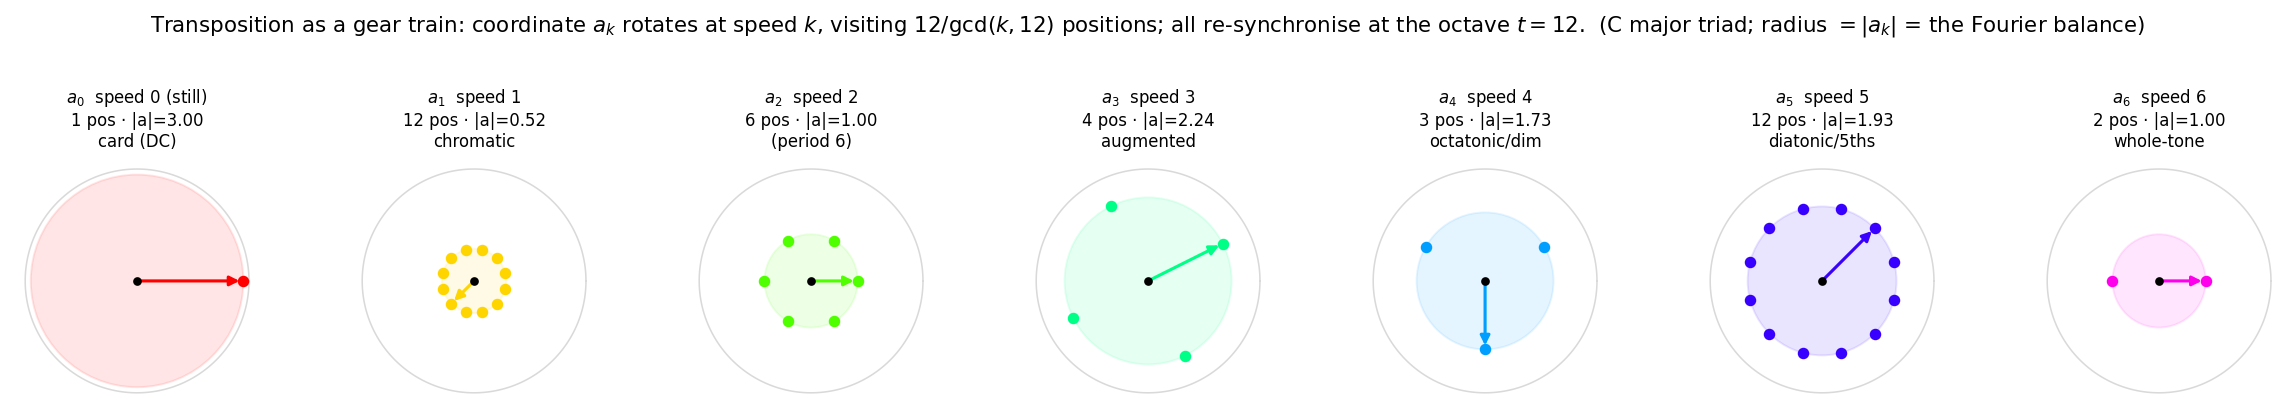
\includegraphics[width=0.74\linewidth]{figs/fig_gears.png}
\caption{Transposition as a gear train: $a_k$ rotates at speed $k$, visiting $12/\gcd(k,12)$ positions; all
re-synchronise at the octave. Radius $=|a_k|$, the Fourier balance ($a_0$ still; $a_3$ augmented $=\sqrt5$;
$a_4$ diminished $=\sqrt3$; $a_6$ whole-tone; the rest as labelled).}
\label{fig:gears}
\end{figure}

\textbf{Inversion folds the basis onto a torus} (Figure~\ref{fig:crttorus}). The Chinese Remainder Theorem
$\Ztwelve\cong\Zn{3}\times\Zn{4}$ ($j\mapsto(j\bmod3,\,j\bmod4)$) splits the universe into two factor circles
--- the \textbf{augmented} axis $\langle4\rangle=\{0,4,8\}$ (the $\Zn3$ factor) and the \textbf{diminished}
axis $\langle3\rangle=\{0,3,6,9\}$ (the $\Zn4$ factor) --- and a chromatic semitone is the diagonal step. On
the dual side the split is exact, with a small but real index flip worth stating precisely.

\begin{proposition}[CRT coordinates of the characters]\label{prop:crt}
Under $\Ztwelve\cong\Zn3\times\Zn4$, a character $\chi_k$ factors through the $\Zn3$ projection iff
$k\in\{0,4,8\}$, and through the $\Zn4$ projection iff $k\in\{0,3,6,9\}$. Hence $\chi_4$ generates the
augmented ($\Zn3$) axis and $\chi_3$ generates the diminished ($\Zn4$) axis, with the tritone $\chi_6$ the
order-$2$ element of the $\Zn4$ part.
\end{proposition}
\noindent\textit{Proof.}~$\chi_k$ factors through $\pi_3:\Ztwelve\to\Zn3$ iff it is trivial on
$\ker\pi_3=\{0,3,6,9\}$, i.e.\ $\chi_k(3)=e^{\pi i k/2}=1$, i.e.\ $4\mid k$; symmetrically through $\pi_4$ iff
$\chi_k(4)=e^{2\pi i k/3}=1$, i.e.\ $3\mid k$.\hfill$\square$

\smallskip\noindent The flip is the point: the augmented triad \emph{maximises} $|a_3|$ because $\chi_3$ is
\emph{constant} on it (it factors through the $\Zn4$ quotient), whereas the character that \emph{resolves}
the augmented axis is $\chi_4$. So ``which scale saturates $a_k$'' and ``which $\chi_k$ coordinatises the
factor'' read off with the indices $3\leftrightarrow4$ swapped --- two dual faces of one CRT splitting.
\emph{Within} a factor circle the points are locked; the diagonal \emph{couples} the two factors into the
single chromatic clock --- the same factor-vs-diagonal that the conjugate-pair blocks of
\S\ref{sec:dihedral} express as counter-rotation vs common drive.

\begin{figure}[H]\centering
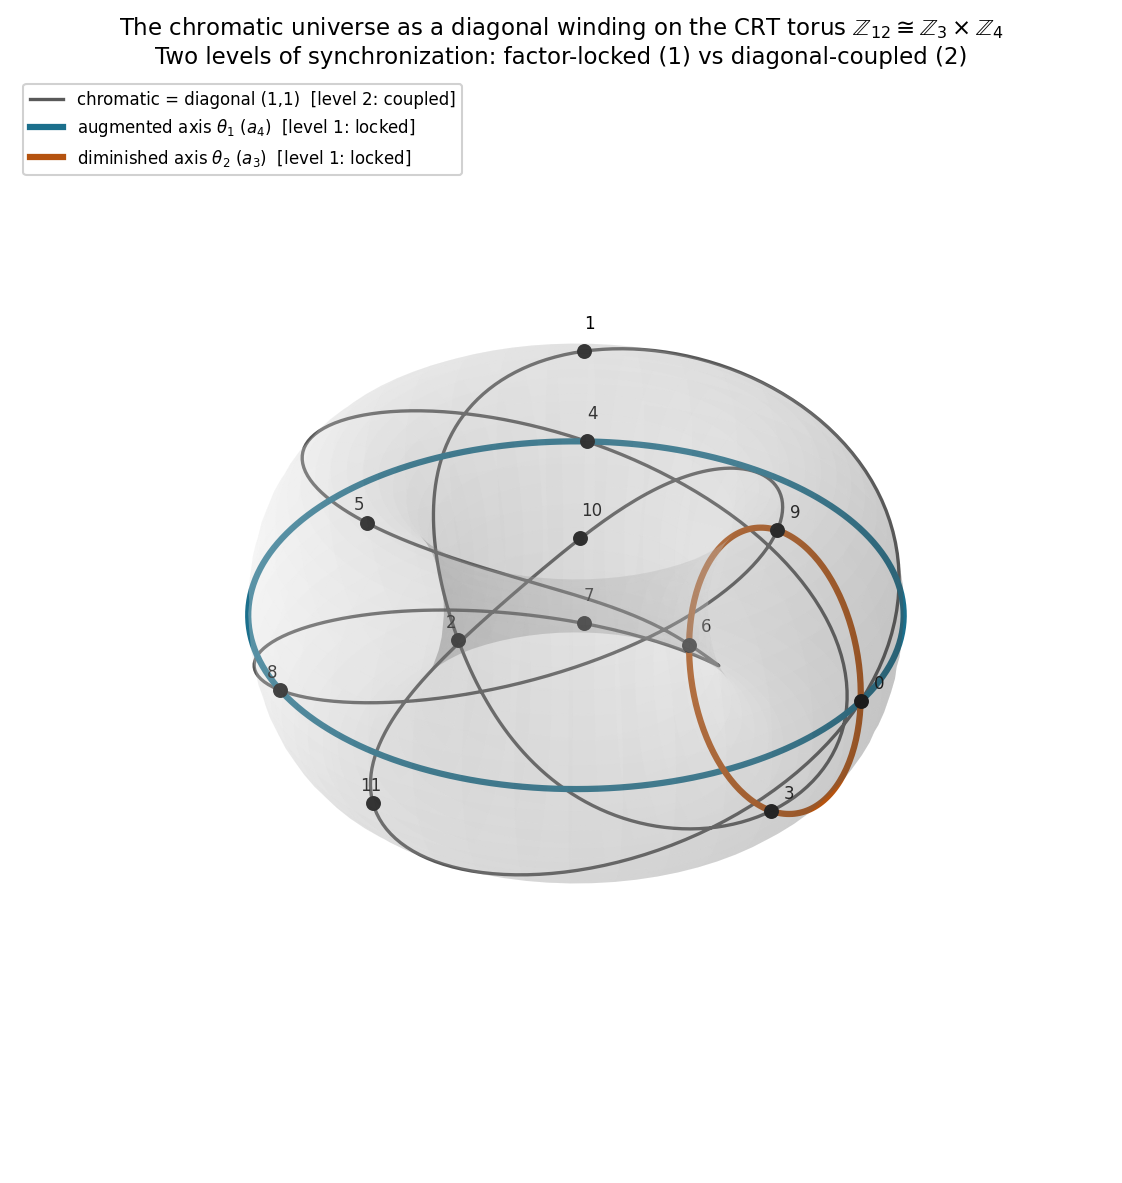
\includegraphics[width=0.62\linewidth]{figs/fig_crttorus.png}
\caption{$\Ztwelve\cong\Zn{3}\times\Zn{4}$ as a diagonal winding on the CRT torus: the factor circles are
the augmented ($\Zn3$, resolved by $\chi_4$) and diminished ($\Zn4$, resolved by $\chi_3$) axes
(Prop.~\ref{prop:crt}); the chromatic is the diagonal. Two levels of synchronisation: factor-locked and
diagonal-coupled.}
\label{fig:crttorus}
\end{figure}

\textbf{Why the tritone seeds every halving.} Before the geometry, the algebra that drives it. Model the
pitch-class circle as $S^1=\mathbb{R}/\mathbb{Z}$; the $2^n$-tone equal temperament is the subgroup
$\mu_{2^n}\cong\Zn{2^n}$ of $2^n$-th roots of unity, and octave bisection nests them
$\Zn{2}\subset\Zn{4}\subset\Zn{8}\subset\cdots$. The map linking one level to the next is the
\textbf{doubling} $\delta:z\mapsto z^2$ (on angles $\theta\mapsto2\theta$), the $2$-to-$1$ octave-folding of
the circle. It is exactly $2$-to-$1$: the fibre of $\delta$ over the unison $z=1$ is
$\{z:z^2=1\}=\{+1,-1\}$, and $-1=e^{\pi i}$ is the \textbf{tritone}, the unique order-$2$ element of $S^1$
(\lean{tritone\_selfPaired}, at every even level). So the binary question at each stage --- ``\emph{which
square root of the unison?}'' --- is precisely ``\emph{unison or tritone?}'': the tritone is the nontrivial
element of every bonding fibre.

\textbf{The dyadic tower: one theorem, and an honest analogy} (Figure~\ref{fig:solenoid}). Iterating the
fibre, the kernels $\ker\delta^{\,n}=\mu_{2^n}\cong\Zn{2^n}$ form a genuine projective system under doubling,
and its inverse limit is a \emph{theorem}, not a metaphor:
$\varprojlim\!\big(\cdots\to\Zn{2^{n+1}}\to\Zn{2^n}\big)\cong\mathbb{Z}_2$, the $2$-adic integers --- the
Cantor fibre of the Smale--Williams solenoid $\mathbb{S}_2=\varprojlim(S^1\xleftarrow{\,\delta\,}S^1\cdots)$,
with the tritone the order-$2$ element at each finite stage and none surviving the torsion-free limit
(geometrically, $\delta$ wraps the solid-torus tube twice around its core; the nested intersection
$\bigcap_n\delta^{\,n}(\text{tube})$ is the attractor). \textbf{What we do \emph{not} claim} is a theorem
identifying the \S\ref{sec:dihedral} block decomposition --- which lives at a single fixed $N$ --- \emph{with}
this solenoid. The tempting route fails cleanly, and we record the negative: the self-paired characters
$\chi_{2^{n-1}}$ are \emph{all} the one sign character $(-1)^j$, so the naive tower of self-paired subspaces
$V_n=\langle\chi_0,\chi_{2^{n-1}}\rangle$ is constant and $\varprojlim V_n$ is merely $\mathbb{C}^2$, not
$\mathbb{S}_2$. We therefore keep the solenoid as a \emph{picture} of the dyadic-grid tower, not as a
corollary of the block theorem; the precise bridge --- a projective system built from the block data and
converging to $\mathbb{S}_2$ --- we flag as \textbf{open} (\S\ref{sec:novelty}). \emph{The solenoid and
$2$-adic-in-music are classical (Pitk\"anen~\cite{Pitkanen}; Fokker~\cite{Fokker}; the $\Zn{4}$/diminished
torus is in Yust~\cite{YustGT}); we add only the doubling-fibre reading of the tritone and the explicit
negative above.}

\begin{figure}[H]\centering
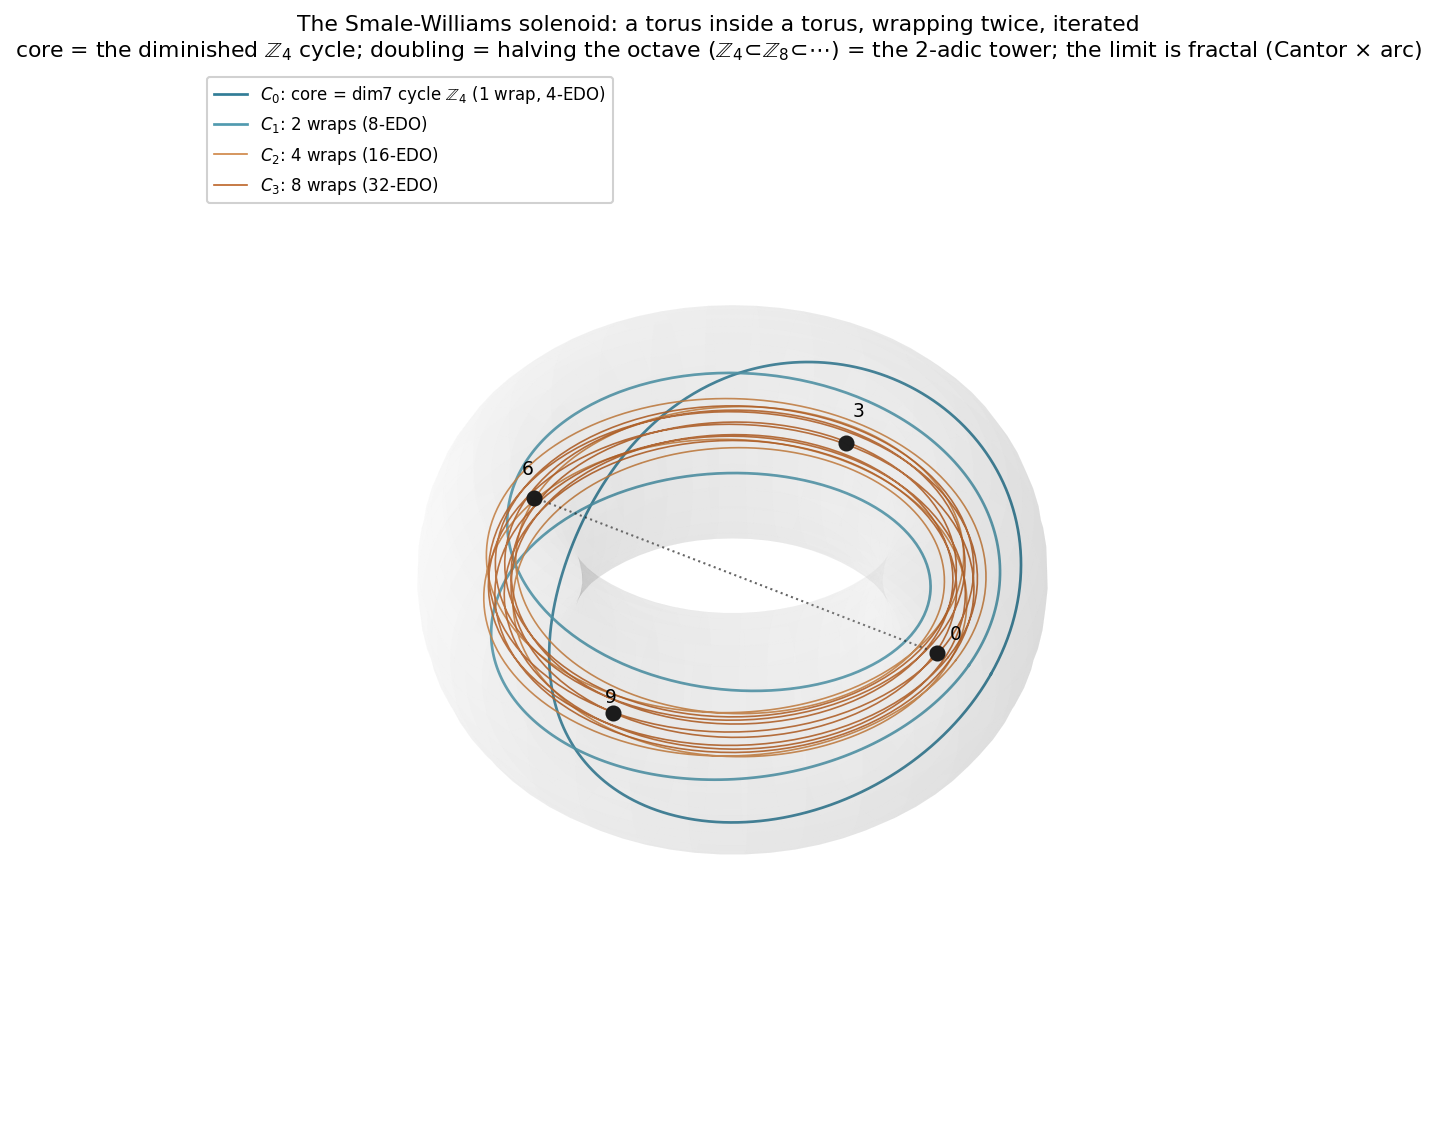
\includegraphics[width=0.66\linewidth]{figs/fig_solenoid.png}
\caption{The Smale--Williams solenoid: a torus wound twice inside a torus, iterated. The doubling
$\delta:z\mapsto z^2$ is $2$-to-$1$, its fibre over the unison being $\{$unison$,$ tritone$\}$; the inverse
limit $\varprojlim(S^1\xleftarrow{\delta}S^1\cdots)$ has a Cantor ($\mathbb{Z}_2$) fibre built from those
binary choices. We use it as a picture of the dyadic-grid tower, not as a corollary of the block theorem
(see text).}
\label{fig:solenoid}
\end{figure}

\qlink{Every step so far has \emph{claimed} a theorem. But a claim is not a proof, and a diagram is not a
certificate. Which of these does a proof kernel actually verify --- and at what axiomatic cost?}

\section{What is machine-checked}\label{sec:checked}

The spectral ladder --- now including completeness --- is certified by the Lean~4 kernel across five
sorry-free files, each with an axiom audit (\lean{\#print axioms}) returning at most
\lean{[propext, Classical.choice, Quot.sound]} and no \lean{sorryAx}; several decidable witnesses are
choice-free. Verified by recompiling each from scratch in the godsil fast-loop environment (EXIT~0).

\begin{table}[!ht]
\centering\footnotesize
\setlength{\tabcolsep}{4pt}
\rowcolors{2}{ctA!7}{white}
\begin{tabular}{@{}p{0.29\textwidth} p{0.195\textwidth} p{0.425\textwidth}@{}}
\toprule
\rowcolor{ctA!22}
\textbf{Theorem} & \textbf{File} & \textbf{Statement}\\
\midrule
\lean{circulant\_mulVec\_dftChar} & \lean{CycleGraphSpectrum} & Every circulant diagonalized by the DFT; eigenvalue $=\hat v(k)$ (keystone).\\
\lean{C12\_eigenvalue\_cos} & \lean{CycleGraphSpectrum} & The $C_{12}$ spectrum is $2\cos(2\pi k/12)$.\\
\lean{C12\_eq\_adjMatrix} & \lean{CycleGraphSpectrum} & $C_{12}$ is Mathlib's \texttt{cycleGraph 12} adjacency matrix.\\
\lean{cayleyAdj\_eigenvalue} & \lean{CycleGraphSpectrum} & Abelian Cayley spectrum $=\sum_{s\in S}\mathrm{stdAddChar}(-(sk))$ (Babai).\\
\lean{inv\_dftChar} / \lean{transl\_dftChar} & \lean{InversionDFT} & Inversion swaps $k\leftrightarrow-k$; translation acts diagonally.\\
\lean{block\_dihedral\_invariant} & \lean{InversionDFT} & The $D_{2N}$ action is block-diagonal (conjugate-pair blocks).\\
\lean{block\_irreducible} & \lean{InversionDFT} & Each $2$-dim block ($k\neq-k$) is an irreducible dihedral irrep.\\
\lean{tritone\_selfPaired} & \lean{InversionDFT} & The tritone is inversion-fixed in every even universe.\\
\lean{powerSpec\_neg} / \lean{IVraw\_eq\_powerSpec\_conjPair} & \lean{Fourier} & $|\Ahat|^2$ constant on conjugate pairs; the interval vector is its fold over $\{k,-k\}$ (the Note~\#2 weld).\\
\lean{A\_mulVec\_ones} / \lean{A\_mulVec\_sign} & \lean{TonnetzSpectrum} & Tonnetz eigenvalues $+3$ and $-3$ (bipartite quality flip).\\
\lean{A\_mulVec\_golden}, \lean{\_j4/j2/j1/j5} & \lean{TonnetzSpectrum} & The full irrational spectrum $\sqrt5,\sqrt3,1,2\cos(\tfrac{\pi}{12}),2\cos(\tfrac{5\pi}{12})$, by explicit eigenvectors.\\
\lean{tonnetz\_spectrum\_\allowbreak complete\_\allowbreak unconditional} & \lean{TonnetzCompleteness} & The $24$ eigenvectors form a \emph{basis} --- completeness: the spectrum is exactly $\{\pm|\hat{\mathbf 1}_T(k)|\}$ (no Sage, no irreps). The named values + multiplicities are the Sage witness.\\
\bottomrule
\end{tabular}
\caption{The spectral ladder, machine-checked across \lean{CycleGraphSpectrum.lean}, \lean{InversionDFT.lean},
\lean{Fourier.lean}, \lean{TonnetzSpectrum.lean} and \lean{TonnetzCompleteness.lean}. Mathlib carries \lean{circulant}, \lean{ZMod.dft},
\lean{cycleGraph}/\lean{circulantGraph} and the dihedral group as \emph{definitions} but no spectrum theorem
and no dihedral-irrep classification; these files supply the spectral layer.}
\label{tab:lean}
\end{table}

\subsection*{Closing the last formal gap: a Mathlib roadmap}
The spectrum is \emph{complete} in Lean without the irrep classification (Table~\ref{tab:lean}, last row): a
DFT-character basis tensored with a quality two-vector suffices. What remains open is only the \emph{named}
isotypic statement --- ``$\mathbb{C}[D_{2N}]\cong\bigoplus_k\rho_k$ as $D_{2N}$-modules'' --- which Mathlib
cannot yet phrase because it has \lean{DihedralGroup N} and \lean{Representation} as definitions but no
classification of dihedral irreducibles. It is a coverage gap, not a hard theorem; the route is three scoped
bricks, in dependency order:
\begin{enumerate}\setlength\itemsep{1pt}
  \item \textbf{The dihedral irreducibles, named.} Build $\rho_k:\lean{DihedralGroup}\,N\to\lean{Matrix (Fin
        2)}\,\mathbb{C}$ ($r\mapsto\mathrm{diag}(\omega^{k},\omega^{-k})$, $s\mapsto$ antidiagonal) and prove
        \lean{IsSimpleModule} for $k\neq-k$. The hard half is already done --- \lean{block\_irreducible} is
        exactly ``no proper invariant subspace''; the brick is the explicit intertwiner
        $\mathrm{block}\,k\;\simeq_{D_{2N}}\;\rho_k$, the constant matrix
        $\tfrac1{\sqrt2}\left(\begin{smallmatrix}1&1\\ i&-i\end{smallmatrix}\right)$.
  \item \textbf{Schur over $\mathbb{C}$ $\Rightarrow$ isotypic \lean{DirectSum}.} With $\rho_k$ named and
        \lean{block\_dihedral\_invariant} giving the block decomposition, Mathlib's finite-dimensional Schur
        (\lean{Module.End} of a simple module is a division ring) packages the regular representation as the
        internal \lean{DirectSum} $\bigoplus_k\mathrm{block}\,k$ with multiplicities $\gcd(2,N)$ ones and the
        rest twos (our \lean{selfPaired\_ncard\_even}).
  \item \textbf{$D_{2N}/Z\cong D_{N}$ for the centralizer (Note~\#1 tie).} The quotient by the centre closes
        the named $\mathrm{Cgrp}\cong D_{6}$ of the $6$-$30$ brick; Mathlib currently offers only
        \lean{center\_eq\_bot\_of\_odd\_ne\_one}, so the even case is the missing lemma.
\end{enumerate}
\noindent Each is standard representation theory; none needs new mathematics. We flag them as the natural
upstreaming targets --- the point at which this note's spectral layer would become reusable Mathlib
infrastructure rather than project-local files.

\section{Novelty, scope, and what this note does not claim}\label{sec:novelty}

\paragraph{Contribution, stated plainly.} This is a formalization-and-organization note, not new
mathematics. Circulant and Cayley-graph spectra are folklore (Godsil--Royle~\cite{GR};
Babai~\cite{Babai}); the $\pm k$ pairing of dihedral irreducibles is standard representation
theory~\cite{Diaconis}; the closed-form dihedral Cayley spectrum is Gao--Luo~\cite{GaoLuo} (of which the
Tonnetz, Theorem~\ref{thm:main}, is the $S=\{P,L,R\}$ instance); the Tonnetz Laplacian was diagonalized by
Lostanlen~\cite{Lostanlen}, the $PLR\cong D_{12}$ duality is Crans--Fiore--Satyendra~\cite{CFS}, the graph is
Douthett--Steinbach~\cite{DS}, the balance dictionary is Quinn--Amiot~\cite{Quinn,Amiot}. What is
\textbf{new} is the \emph{unified, machine-checked} account, and within it the \textbf{first formalization in
any proof assistant} of: (i)~the circulant diagonalization-by-DFT and the abelian-Cayley spectrum;
(ii)~the DFT-basis block decomposition of the $D_{2N}$ action and the $2$-dimensional block irreducibility
--- the dihedral representation theory on pitch classes; (iii)~explicit eigenvectors certifying the entire
Tonnetz spectrum --- the $S=\{P,L,R\}$ instance of the Gao--Luo formula~\cite{GaoLuo}, here machine-checked.
All are made universe-generic. Beyond formalization, one \emph{expository} identification appears
unstated: (iv)~that the Tonnetz adjacency spectrum is the triad's own Fourier-balance multiset
(\S\ref{sec:tonnetz}); its components are classical, the weld is the contribution.

\paragraph{What this note does \emph{not} claim.}
\begin{itemize}\itemsep2pt
  \item \textbf{Not new mathematics.} First \emph{formalization} and \emph{organization} only.
  \item \textbf{Not a new formalization of the $T/I$ action.} Prismriver~\cite{Prismriver} (Lean~4)
        formalizes the bare $D_{2N}$ action on pitch classes; we cite it and claim only the Fourier-basis
        \emph{representation theory} and the circulant/Cayley spectrum, which it does not treat (confirmed by
        a file-by-file audit: no DFT/character/circulant/irrep content).
  \item \textbf{Complete in Lean, but not via the irrep classification.} The spectrum is now \emph{complete}
        in Lean --- the $24$ eigenvectors form a certified basis
        (\lean{tonnetz\_spectrum\_\allowbreak complete\_\allowbreak unconditional}),
        a full diagonalization --- yet \emph{not} by the $D_{12}$ isotypic decomposition (Mathlib lacks it);
        completeness comes instead from DFT-character $\otimes$ quality-pair independence. The named
        dihedral-irrep isomorphism remains the one open formal item.
  \item \textbf{Not a golden-ratio mystery --- but $\sqrt5$ \emph{is} the augmented balance.} As a bare
        identity $|1+2i|=\sqrt5$ occurs whenever $4\mid n$; its musical content is that $\sqrt5=|a_3|$ is the
        triad's augmented balance (its largest non-trivial Fourier component), the slowest-mixing harmonic
        mode (spectral gap $3-\sqrt5$).
  \item \textbf{Not first-contact for $2$-adic music.} The dyadic-tower/solenoid remark (\S\ref{sec:geometry})
        is expository; Pitk\"anen~\cite{Pitkanen} and Fokker~\cite{Fokker} precede it, and we cite them.
\end{itemize}

\paragraph{Open frontier.} The named dihedral-irrep isomorphism and the isotypic decomposition (pending a
Mathlib classification) --- now the \emph{only} remaining formal gap, since spectral completeness is
machine-checked (\S\ref{sec:tonnetz}); and the literal cross-file welding of the conjugate pair to the
index-vector fold of Note~\#2.

\section*{Coda: questions the eigenbasis leaves open}
We began with one basis and followed it across three symmetries. The picture it leaves is unreasonably tidy
--- tidy enough to make one ask what that tidiness is really saying.

\qlink{If a single basis diagonalizes transposition, inversion, \emph{and} the neo-Riemannian group at once,
is a style's ``colour'' just a choice of which Fourier balance to maximize --- and could a working theory of
harmony be rebuilt, from the balance profile up, rather than from the chord down?}

\qlink{The tritone is the unique self-paired frequency in every even universe --- the one fixed point the
symmetry cannot move, the singularity that forces the blocks. Is its long history as the
\emph{diabolus in musica} a cultural echo of a structural fact, the ear hearing an algebraic invariant
centuries before it could be named?}

\qlink{Completeness needed no $D_{12}$ irrep classification --- a character basis tensored with a
two-vector sufficed. Where else does a ``hard'' representation-theoretic theorem quietly dissolve into linear
algebra, the moment the right basis is written down?}

\section*{Data and code availability}
\begin{sloppypar}
The Lean sources \lean{CycleGraphSpectrum.lean}, \lean{InversionDFT.lean}, \lean{TonnetzSpectrum.lean},
\lean{TonnetzCompleteness.lean} (the completeness basis), \lean{Fourier.lean}, the Sage script
\lean{tonnetz\_cayley\_spectrum.py} (load-bearing for the named factored characteristic polynomial and its
multiplicities, which Lean does not evaluate --- the Lean basis certifies completeness as the multiset
$\{\pm|\hat{\mathbf 1}_T(k)|\}$, the Sage witness identifies it with the named values), the microtonal
\lean{z24\_saturation.sage} (exact cyclotomic), and the figure scripts in \lean{viz/} accompany this note; each Lean theorem is checkable by
\lean{\#print axioms} and compiles axiom-clean (only \lean{propext}, \lean{Classical.choice},
\lean{Quot.sound}).
\end{sloppypar}

\appendix
\section{The spectrum as a generative engine}
\label{app:compose}

The note reads scales and chords \emph{forward}: a pc-set $A\subseteq\Zn{N}$ has a Fourier profile
$|a_k(A)|$, $a_k(A)=\sum_{j\in A}e^{-2\pi i kj/N}$, and the largest $|a_k|$ names its colour (augmented at
$k{=}3$, octatonic at $k{=}4$, whole-tone at $k{=}6$). Composition is the \emph{inverse} problem: fix a
colour $k$, and let the algebra hand back the set that saturates it. This is the practical face of
``composing in Fourier space'' (Amiot~\cite{Amiot}, ch.~on composition); we record the exact rule and the
audio it produced.

\textbf{The saturation rule (exact).} For a set of cardinality $d$, $|a_k(A)|\le d$, with equality iff all
phases coincide, i.e.\ $k\!\cdot\!A$ is constant in $\Zn{N}$ --- iff $A$ lies in a single coset of
\[
  H_k \;=\; \ker\bigl(j\mapsto kj\bigr) \;=\; \tfrac{N}{\gcd(N,k)}\,\Zn{N},
  \qquad |H_k|=\gcd(N,k).
\]
So the \emph{maximal}-$|a_k|$ set of cardinality $\gcd(N,k)$ is exactly a coset $c+H_k$, and its balance is
$|a_k|=\gcd(N,k)$. In $\Zn{12}$ this is precisely Messiaen's catalogue of \emph{modes of limited
transposition}~\cite{Messiaen}: $H_3=\{0,4,8\}$ the augmented triad, $H_4=\{0,3,6,9\}$ the diminished
seventh, $H_6=\{0,2,4,6,8,10\}$ the whole-tone scale. When $\gcd(N,k)=1$ (e.g.\ $k{=}5,1$ in $\Zn{12}$)
there is no nontrivial coset, and the maximiser of $|a_k|$ over a chosen cardinality is instead the
\emph{maximally even} set (Clough--Douthett~\cite{CloughDouthett}; Amiot) --- the diatonic for $k{=}5$.

\textbf{Algorithm (reproducible).}
\begin{enumerate}\setlength\itemsep{0pt}
  \item Pick a colour $k\in\Zn{N}$ and a length $L$.
  \item If $\gcd(N,k)>1$: seed $\leftarrow$ a coset $c+H_k$ (a Messiaen mode, $|a_k|$ saturated);
        else seed $\leftarrow$ a maximally even set of the chosen cardinality.
  \item Voice-lead by walking the Tonnetz with conjugate-pair-preserving moves (PLR$\,\cong D_{12}$): each
        triad's neighbourhood spectrum is \emph{its own} colour profile (\S\ref{sec:tonnetz}), so the walk
        keeps the harmony inside the chosen Fourier band.
  \item Emit $L$ pitch-classes traversing the seed and its Tonnetz orbit.
\end{enumerate}

\begin{table}[h]\centering\footnotesize\setlength{\tabcolsep}{5pt}
\rowcolors{2}{ctA!8}{white}
\begin{tabular}{@{}p{0.10\textwidth} p{0.13\textwidth} p{0.31\textwidth} p{0.30\textwidth}@{}}
\toprule
\rowcolor{ctA!22}
\textbf{Colour $k$} & \textbf{$|a_k|$} & \textbf{Saturating set $=c+H_k$} & \textbf{Realisation}\\
\midrule
$3$ & $\sqrt5\,$(triad)$,\;3$ & augmented triad $\{0,4,8\}$ & \lean{augmented\_cycle.wav}\\
$4$ & $\sqrt3\,$(triad)$,\;4$ & diminished seventh $\{0,3,6,9\}$ & \lean{petrushka\_octatonic.wav}\\
$6$ & $1\,$(triad)$,\;6$ & whole-tone $\{0,2,4,6,8,10\}$ & \lean{modes\_messiaen.wav}\\
$5$ & $2\cos\frac{\pi}{12}$ & diatonic (maximally even, no coset) & \lean{tonnetz\_hexatonic.wav}\\
even $k$ & $2$ & tritone axis $\{0,6\}$, the $2$-torsion & \lean{tritone\_symmetry.wav}\\
\bottomrule
\end{tabular}
\end{table}

\textbf{Microtonal instance ($N=24$, quarter tones).} The saturation rule is $N$-generic --- $H_k$ and
$|a_k|=\gcd(N,k)$ are stated over an arbitrary universe, the same parametrisation the Lean
\lean{selfPaired\_even}/\lean{tritone\_selfPaired} carry over all $N$ (\S\ref{sec:dihedral}). Reading it at
$N=24$ produces the quarter-tone catalogue of limited-transposition modes, and that catalogue \emph{strictly
extends} the chromatic one: the tritone fixed point migrates to $q=N/2=12$, and one mode --- $H_8$ --- lands
on \emph{odd} quarter tones, with no $12$-TET analogue.

\begin{table}[h]\centering\footnotesize\setlength{\tabcolsep}{5pt}
\rowcolors{2}{ctB!8}{white}
\begin{tabular}{@{}p{0.07\textwidth} p{0.07\textwidth} p{0.40\textwidth} p{0.30\textwidth}@{}}
\toprule
\rowcolor{ctB!22}
\textbf{$k$} & \textbf{$|a_k|$} & \textbf{Saturating coset $H_k\subseteq\Zn{24}$ (quarter tones)} & \textbf{$12$-TET reading}\\
\midrule
$3$  & $3$  & $\{0,8,16\}$ & augmented triad (even grid)\\
$4$  & $4$  & $\{0,6,12,18\}$ & diminished seventh (even grid)\\
$6$  & $6$  & $\{0,4,8,12,16,20\}$ & whole-tone scale (even grid)\\
$8$  & $8$  & $\{0,3,6,9,12,15,18,21\}$ & \textbf{off-grid} --- a genuinely $24$-TET mode\\
$12$ & $12$ & $\{0,2,4,\dots,22\}$ & the full chromatic scale\\
\bottomrule
\end{tabular}
\end{table}

\noindent Audio: \lean{microtonal\_z24.wav} sounds the five cosets in 24-EDO (additive sines at
$f_0\,2^{q/24}$; a quarter tone is not a $12$-TET MIDI semitone, so this one is WAV-only). $H_8$ is the
audible payoff --- a symmetric mode the chromatic scale cannot voice.

\textbf{Scope (honest).} The construction is not new mathematics: the coset-saturated sets \emph{are}
Messiaen's limited-transposition modes, and maximal evenness is Clough--Douthett / Amiot. What this appendix
adds is the unifying reading --- \emph{composition = choosing which Fourier balance to saturate, after which
the subgroup $H_k$ (or maximal evenness) dictates the material} --- together with the Tonnetz-spectrum tie
(\S\ref{sec:tonnetz}: a generated triad's adjacency spectrum returns its own balances) and the reproducible
audio. It is an illustration that the forward spectral theory of this note is also generative; it is not a
compositional theory in its own right.

\begin{thebibliography}{99}
\bibitem{Amiot} E. Amiot, \emph{Music Through Fourier Space: Discrete Fourier Transform in Music Theory},
  Computational Music Science, Springer, 2016.
\bibitem{Babai} L. Babai, ``Spectra of Cayley graphs,'' \emph{J. Combin. Theory Ser. B} \textbf{27} (1979),
  180--189.
\bibitem{CFS} A. Crans, T. Fiore, R. Satyendra, ``Musical actions of dihedral groups,'' \emph{Amer. Math.
  Monthly} \textbf{116} (2009), no.~6, 479--495 (arXiv:0711.1873).
\bibitem{CloughDouthett} J. Clough, J. Douthett, ``Maximally even sets,'' \emph{J. Music Theory}
  \textbf{35} (1991), no.~1/2, 93--173.
\bibitem{Messiaen} O. Messiaen, \emph{Technique de mon langage musical}, Alphonse Leduc, Paris, 1944
  (modes of limited transposition).
\bibitem{Diaconis} P. Diaconis, \emph{Group Representations in Probability and Statistics}, IMS Lecture Notes
  \textbf{11}, 1988.
\bibitem{DS} J. Douthett, P. Steinbach, ``Parsimonious graphs: a study in parsimony, contextual
  transformations, and modes of limited transposition,'' \emph{J. Music Theory} \textbf{42} (1998), no.~2,
  241--263.
\bibitem{Fokker} A. D. Fokker, ``Unison vectors and periodicity blocks\dots,'' \emph{Proc. Kon. Ned. Akad.
  Wetensch.} \textbf{B72} (1969), 153--168.
\bibitem{GR} C. Godsil, G. Royle, \emph{Algebraic Graph Theory}, GTM \textbf{207}, Springer, 2001.
\bibitem{GaoLuo} X. Gao, Y. Luo, ``The spectrum of semi-Cayley graphs over abelian groups,'' \emph{Linear
  Algebra Appl.} \textbf{432} (2010), no.~11, 2974--2983.
\bibitem{LiuSurvey} X. Liu, S. Zhou, ``Eigenvalues of Cayley graphs,'' survey, arXiv:1809.09829
  (the dihedral case is Theorem~51).
\bibitem{Abdollahi} A. Abdollahi, S. Janbaz, M. Ghahramani, ``A large family of cospectral Cayley graphs over
  dihedral groups,'' \emph{Discrete Math.} \textbf{340} (2017), no.~5, 1116--1121 (the cospectrality from the
  difference multiset is Babai~\cite{Babai}, Cor.~4.2).
\bibitem{Loeffler} D. Loeffler, Mathlib \lean{ZMod.dft} (Apache-2.0) --- the discrete Fourier transform on
  \lean{ZMod N} as a \lean{LinearEquiv}.
\bibitem{Lostanlen} V. Lostanlen, ``Eigentriads and eigenprogressions on the Tonnetz,'' ISMIR 2018
  (arXiv:1810.00790).
\bibitem{MGAAA} J. Mandereau, D. Ghisi, E. Amiot, M. Andreatta, C. Agon, ``Z-relation and homometry in
  musical distributions,'' \emph{J. Math. \& Music} \textbf{5} (2011), no.~2, 83--98.
\bibitem{Pitkanen} M. Pitk\"anen, ``2-adic numbers and music scales,'' online note, 1999.
\bibitem{Prismriver} L. Aniva, C. Wang, \emph{Prismriver}, arXiv:2606.19936 --- Lean~4 formalization of the
  $T/I$ action on pitch-class sets.
\bibitem{Quinn} I. Quinn, ``General equal-tempered harmony,'' \emph{Perspectives of New Music}
  \textbf{44}--\textbf{45} (2006--2007).
\bibitem{YustGT} J. Yust, ``Generalized Tonnetze and Zeitnetze, and the topology of music concepts,''
  \emph{J. Math. \& Music} \textbf{14} (2020), no.~2 (arXiv:1612.03519).
\bibitem{Note1} C. Mar\'in, ``A tritone-centered self-duality: the set class 6-30 and its order-12
  neo-Riemannian dual,'' Note~\#1 (music-math series), 2026 (DOI:10.5281/zenodo.20820962).
\bibitem{Note2} C. Mar\'in, ``The phase taxonomy of pitch-class set invariants,'' Note~\#2 (music-math
  series), 2026 (DOI:10.5281/zenodo.20826774).
\end{thebibliography}

\end{document}
